\documentclass{beamer}
%\usetheme{CambridgeUS}
\usetheme{Warsaw}

\usepackage[utf8]{inputenc}
\usepackage{pgfpages}
\usepackage{outlines}
\usepackage{xcolor} 

\usepackage{hyperref}
\makeatletter

%\Hy@AtBeginDocument{%
%  \def\@pdfborder{0 0 1}% Overrides border definition set with colorlinks=true
%  \def\@pdfborderstyle{/S/U/W 1}% Overrides border style set with colorlinks=true
%                                % Hyperlink border style will be underline of width 1pt
%}
\makeatother
\hypersetup{
%    colorlinks=true,
%    linkcolor=cyan,
%    linkbordercolor=cyan,
%    urlcolor=cyan,
%    urlbordercolor=cyan
}

\usepackage{soul}
\usepackage{color}

\makeatletter
\let\HL\hl
\renewcommand\hl{%
  \let\set@color\beamerorig@set@color
  \let\reset@color\beamerorig@reset@color
  \HL}
\makeatother

\usepackage{enumitem}
\setitemize{label=\usebeamerfont*{itemize item}%
  \usebeamercolor[fg]{itemize item}
  \usebeamertemplate{itemize item}}
\setenumerate[1]{%
  label=\protect\usebeamerfont{enumerate item}%
        \protect\usebeamercolor[fg]{enumerate item}%
        \insertenumlabel.}
  
%\setbeameroption{show notes on second screen}
%\setbeameroption{hide notes}
%\setbeameroption{show only notes}

\setbeamertemplate{headline}{}
\setbeamertemplate{navigation symbols}{}
\setbeamertemplate{section in toc}[ball]
\setbeamertemplate{subsection in toc}[ball numbered]
\setbeamertemplate{itemize items}[square]
\setbeamertemplate{enumerate items}[square]

\title{Generating pentest reports with Reconmap}
\subtitle{CyberScotland Week}
\author[]{Santiago Lizardo}
\date{February 26, 2021}

\begin{document}

\begin{frame}
    \note[item]{
    }
    
	
\includegraphics[width=\textwidth]{cyberscotland-week-reconmap.jpg}
	\maketitle
\end{frame}


\begin{frame}
    \frametitle{Before the talk}
    
    \note[item]{
    }

    \begin{itemize}
    		\item Time for Q\&A
    		\item Slides
    		\item Survey
    \end{itemize}
\end{frame}

\begin{frame}
	\frametitle{Agenda}
	
		\note[item]{
	}
	
	\tableofcontents[hideothersubsections]
\end{frame}

\begin{frame}
    \frametitle{About the presenter}
    
    \note[item]{
    }

	\begin{columns}
		\begin{column}{0.5\textwidth}
	    \begin{itemize}
	    		\item Software engineer and entrepreneur
	    		\item Based in Scotland
	    		\item Security advocate
	    		\item Reconmap's founder
	    \end{itemize}
		\end{column}

		\begin{column}{0.5\textwidth}
		
\includegraphics[width=0.6\textwidth]{santiago-lizardo-presenter.png}
		\end{column}
	\end{columns}
\end{frame}

\begin{frame}
    \frametitle{Imposter syndrome}
    
    	\begin{figure}[h]
	\centering
	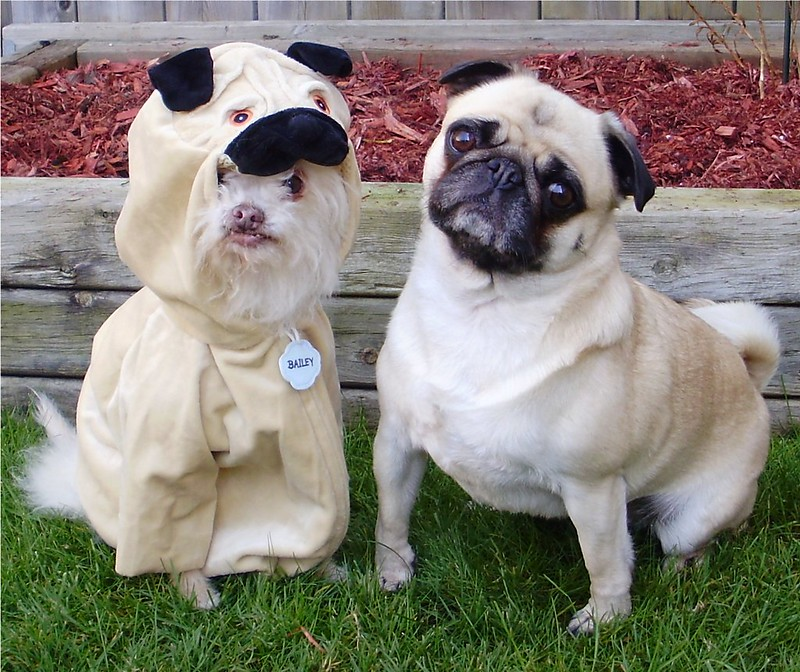
\includegraphics[width=0.8\textwidth]{imposter-syndrome.jpg}
	\caption{https://flic.kr/p/dQC9kt}
	\end{figure}
\end{frame}

\section{Basic pentesting concepts}

\begin{frame}
    \frametitle{Section outline}

    \tableofcontents[currentsubsection, hideothersubsections, sectionstyle=show/hide]
\end{frame}


\begin{frame}
    \frametitle{Vulnerability assessment}
    
    \note[item]{
    }
    
    \begin{itemize}
    		\item Assess security of network or apps
    		\item Identifies vulnerabilities
    		\item Involves scanning tools
    		\item Produces a report
    \end{itemize}

    \pause
    
    \begin{alertblock}{False positives}
	Findings are not exploited, some of them could just be false positives.
    \end{alertblock}
\end{frame}

\subsection{Pentest definition}

\begin{frame}
    \frametitle{Pentest definition}

    \note[item]{
    }

	\begin{itemize}
    		\item Assess security of network or apps
    		\item Identifies vulnerabilities
    		\item Use scanning tools
		\item \textbf{Vulnerabilities are carefully exploited}
    		\item Produces a report
	\end{itemize}	    
\end{frame}

\begin{frame}
    \frametitle{Pentest definition (continued)}

    \note[item]{
    }

	\begin{itemize}
		\item Systematic process
		\item Defined scope
		\item Legal
		\item Authorised
	\end{itemize}	    
\end{frame}

\begin{frame}
    \frametitle{Types of pentesting}

    \note[item]{
    }

	\begin{figure}
		\centering	
		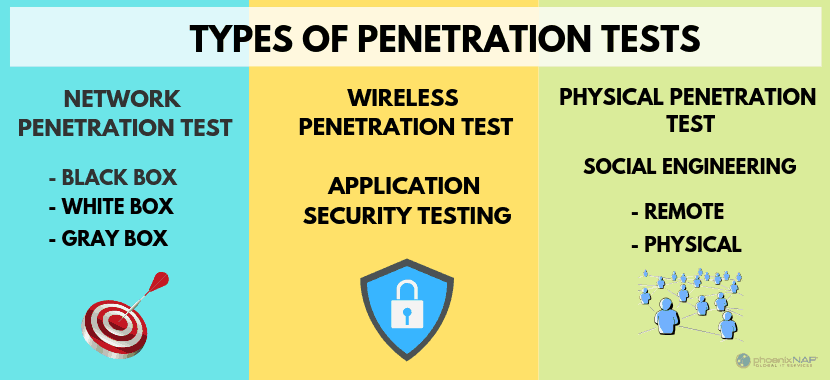
\includegraphics[width=\linewidth]{types-of-pen-testing.png}
		\caption{Source phoenixnap.com}
	\end{figure}    
\end{frame}

\subsection{Objectives and benefits of pentesting}

\begin{frame}
    \frametitle{Pentesting objectives}
    
    \note[item]{
    }
    
    	\begin{itemize}
    		\item Depict the current security level
    		\item Identify gaps
    		\item Quantify potential damage
		\item Validate/Invalidate security controls
    		\item Decreases the possibility of real attacks
    	\end{itemize}
\end{frame}

\begin{frame}
    \frametitle{Business benefits}
    
    \note[item]{
    }
    
    	\begin{outline}
    		\1 Helps with compliance
    			\2 ISO27001
    			\2 PCI DSS
    			\2 HIPPA
    			\2 GLBA
    			\2 FISMA/NIST
    		\1 Protects staff, customers and business partners
    		\1 Preserves company reputation
    		\1 Helps sustain business continuity
    	\end{outline}
\end{frame}

\begin{frame}
    \frametitle{Cost of a pentest}
    
    \note[item]{
    }
    
    \begin{table}
    \begin{tabular}{l | r}
    Test size & Guide price\footnotemark\\
    \hline
    Small & £1000-£3000\\
    Medium & £3000-£5000\\
    Large & £5000-£20000\\        
    \end{tabular}
    \end{table}
	\pause
    	\begin{alertblock}{Cost}
    		Data breaches costed £2.9M to orgs in 2020
    	\end{alertblock}
    
    	\footnotetext[1]{Source \url{bulletproof.co.uk}}
\end{frame}

\begin{frame}
    \frametitle{Engagement length}
    
    \note[item]{
    }
    
    	\begin{itemize}
    		\item Typical engagements are 1 to 3 weeks*
    	\end{itemize}
  	\pause
    	\begin{alertblock}{Recovery time}
    		Orgs take 280 days on average to detect and respond to an incident.\footnotemark[1]
    	\end{alertblock}
    	
    	\footnotetext[1]{https://www.itgovernance.co.uk/blog/the-cost-of-a-data-breach-in-2020}
\end{frame}

\begin{frame}
    \frametitle{When to perform a pentest}
    \framesubtitle{Reactively}
    
    \note[item]{
    }
    
    	\begin{itemize}
    		\item Prior to contracting a data breach insurance
    		\item Before and after corporate milestones
    		\item After noticing viruses, malware, spyware on the system
    		\item After noticing unusual system patterns, traffic
    		\item After system change \& new system deployments
    		\item After new system integrations
    		\item After the release of new products/features    		
    	\end{itemize}
\end{frame}

\begin{frame}
    \frametitle{When to perform a pentest}
    \framesubtitle{Proactively}
        
    \note[item]{
    }

	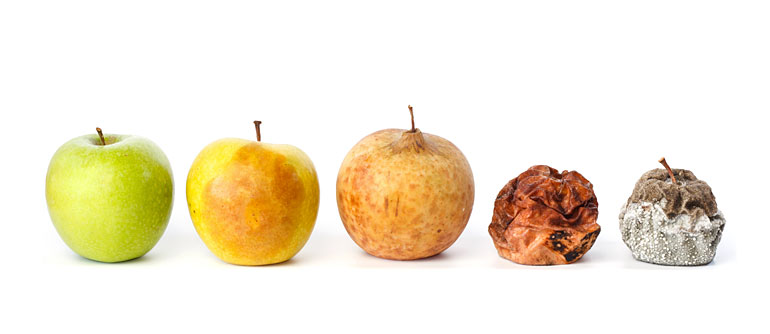
\includegraphics[width=\linewidth]{rotten-apples.jpg}    
    
    	\begin{itemize}
    		\item Regularly as a preventive measure    	
    		\item At least once a year
    	\end{itemize}
\end{frame}

\subsection{The pentesting methodology}

\begin{frame}
    \frametitle{Penetration testing standards}

    \note[item]{
    }
    
	\begin{itemize}
		\item OSSTMM
		\item OWASP
		\item NIST
		\item PTES
		\item ISSAF		
	\end{itemize}	    
\end{frame}

\begin{frame}
    \frametitle{Pentesting workflow}

    \note[item]{
        }
        
	\begin{outline}
		\1 Pre-engagement, analysis and plan
		\1 Information gathering and reconnaissance
		\1 Discovering vulnerabilities
		\1 Exploitation
			\2 Gaining access
			\2 Privilege escalation
			\2 Maintaining access
			\2 Covering tracks
		\1 Analysis and reporting
		\1 Re-test (aka post-fix verification)
	\end{outline}
\end{frame}

\begin{frame}
    \frametitle{Pre-engagement}

    \note[item]{
    }
    
	\begin{outline}
		\1 Paperwork
			\2 Rules of engagement
			\2 Contract
			\2 NDA
		\1 Documentation sharing
		\1 Setup	
			\2 Sharing credentials
			\2 Lifting restrictions
			\2 ...
	\end{outline}	    
\end{frame}

\begin{frame}
    \frametitle{Determine scope}

    \note[item]{
    }
    
	\begin{outline}
		\1 Targets
			\2 Web app
			\2 Mobile apps
			\2 Database
			\2 Network
			\2 Wireless
		\1 End user and social engineering attacks
		\1 DDos and performance tests
		\1 Internal/External
		\1 Physical/Remote
	\end{outline}	    
\end{frame}

\begin{frame}
    \frametitle{Determine scope (continued)}

    \note[item]{
    }
    
	\begin{itemize}
		\item Testing hours/days (eg workdays vs weekends)
		\item Locations
		\item Network range
		\item Teams
	\end{itemize}	    
\end{frame}


\begin{frame}
    \frametitle{Analysis and reporting}

    \note[item]{
    }
    
    Typical report
    
	\begin{itemize}
		\item Summary
		\item Findings
		\item Recommendations
		\item Methodology				
	\end{itemize}	    

	Communication	
	\begin{itemize}
		\item Executive summary delivered to leadership
		\item Project closure meeting organised to discuss
	\end{itemize}	    

\end{frame}

\begin{frame}
    \frametitle{Analysis and reporting (examples)}

    \note[item]{
    }

	Pentest report examples $\rightarrow$ \url{https://pentestreports.com}    
	
	\begin{itemize}
		\item Over 150 example reports
		\item Stored on Github
		\item Source of learning and inspiration
	\end{itemize}
\end{frame}

\begin{frame}
    \frametitle{Re-test}

    \note[item]{
    }
    
	\begin{itemize}
		\item The company is expected to close the gaps
		\item After the gap-closure, a time frame is determined by both parties for verification tests
		\item Findings in the report are reevaluated in the verification tests
	\end{itemize}	    
\end{frame}

\subsection{The role of the pentester}

\begin{frame}
    \frametitle{Pentester}

    \note[item]{
    }
    
    \begin{itemize}
    		\item Plans and designs penetration tests
    		\item Carry out tests and other simulations
    		\item Creates reports and offer recommendations
    		\item Advises management on security improvements
    		\item Work with other employees to improve organizational cybersecurity
    \end{itemize}
\end{frame}

\begin{frame}
    \frametitle{Pentester tools}

    \note[item]{
    }
    
    \begin{itemize}
    		\item From notebooks and post its to text files and wikis
    		\item (Power)Shell scripts
    		\item Security tools (Zap, Burp, nmap, ...)
    		\item Jira/Trello/Gitlab, ...
    		\item Word/Libreoffice
    		\item Email/Chat    		
    \end{itemize}
\end{frame}

\begin{frame}
    \frametitle{Becoming a pentester}

    \note[item]{
    }
    
	\begin{outline}
		\1 Courses
		\1 University degress
			\2 Computer science
			\2 Ethical hacking/Cybersecurity
				\3 \href{https://www.abertay.ac.uk/course-search/undergraduate/cybersecurity/}{Abertay University}
		\1 Practice, practice practice
	\end{outline}
\end{frame}

\begin{frame}
    \frametitle{Becoming a pentester (continued)}

    \note[item]{
    }
    
	\begin{outline}
		\1 Capture the flag/Interactive
		\2 Hackthebox.eu
		\2 PentesterLab.com
		\2 VirtualHackingLabs.com
		\1 Cybrary
		\1 PentesterAcademy
	\end{outline}
	
	\begin{exampleblock}{Bug bounty programs}
	To receive recognition and compensation for reporting bugs, especially those pertaining to security exploits and vulnerabilities.
	\end{exampleblock}
\end{frame}

\begin{frame}
    \frametitle{Becoming a pentester (continued)}
    \framesubtitle{Certifications}

    \note[item]{
    Certified Ethical Hacker
    Licensed Penetration Tester
    Offensive Security Certified Professional
    Offensive Security Certified Expert
    }

	\begin{outline}
		\1 EC-Council CEH and LPT
		\1 IACRB CPT and CEPT
		\1 OSCP, OSCE
		\1 CREST Practitioner, Registered, Certified Tester
		\1 CompTIA PenTest+
	\end{outline}
\end{frame}


\section{Reconmap's introduction}

\begin{frame}
    \frametitle{Section outline}

    \tableofcontents[currentsubsection, hideothersubsections, sectionstyle=show/hide]
\end{frame}

\subsection{Reconmap's mission}

\begin{frame}
    \frametitle{Reconmap mission}

    \note[item]{
    }
    
	\huge{\textbf{Reconmap} is making of \hl{every software engineer a penetration tester}}
\end{frame}

\begin{frame}
    \frametitle{Reconmap mission}

    \note[item]{
    }
    
    \centering
    
\includegraphics[scale=0.6]{oh-really.png}
\end{frame}

\begin{frame}
    \frametitle{Reconmap mission (continued)}

    \note[item]{
    }
    
    \begin{itemize}
    \item Make security testing more accessible
	\item Help (infosec)engineers collaborate better
    \item Accelerate project delivery
    \item Maximise returns
    \end{itemize}
\end{frame}

\begin{frame}
    \frametitle{What is Reconmap?}

    \note[item]{
    }
    
    \begin{outline}
	\1 Collaboration platform for InfoSec projects    
	\1 Automation and reporting tool for pentesters
	\1 Also...
    \2 Early-stage project
	\2 Open-source and SaaS
    \2 Developed in Dundee\footnotemark[1]
    \end{outline}
    
    \footnotetext[1]{with contributions from Argentina and the world}
\end{frame}

\begin{frame}
    \frametitle{Who is it for?}

    \note[item]{
    }
    
    \begin{outline}
	\1 InfoSec pros and teams looking to become more efficient
	\1 Other technical minded people\footnotemark[1] wanting to
	\2 Learn about security
    \2 Perform basic security on their projects
    \end{outline}
    
	\footnotetext[1]{devs, devops, it admins, sys admins, qa, etc...}
\end{frame}

\subsection{Features}

\begin{frame}
    \frametitle{Reconmap's functionality}

    \note[item]{
    }
    
    \begin{outline}
	\1 Project/Methodology templating
	\1 Task management
	\1 Shared space for
		\2 Files (docs, results, screenshots, etc)
		\2 Notes
	\1 Automation tool
    \end{outline}
\end{frame}


\begin{frame}
    \frametitle{Features}

    \note[item]{
    }
    
    \begin{outline}  		
    		\1 Database
    			\2 Commands
    			\2 Vulnerabilities
    			\2 Notes
    			
    		\1 Command automation
    		\1 Report generator
    \end{outline}
\end{frame}

\begin{frame}
    \frametitle{Commands}

    \note[item]{
    }
    \begin{columns}
		\begin{column}{0.5\textwidth}
			\begin{block}{Custom commands}
			\begin{itemize}
				\item Any arbitrary command
				\item Exec and dependencies installed by the user
				\item No upload integration
			\end{itemize}
			\end{block}
		\end{column}
		\begin{column}{0.5\textwidth}
			\begin{block}{Rmap commands}
			\begin{outline}
				\1 Container based
				\1 Dependencies included
	    			\1 Portable to Windows/Macos/Linux
	    			\1 Tighter integration with dashboard
		    \end{outline}
		    \end{block}
		\end{column}
	\end{columns}

\end{frame}

\begin{frame}
    \frametitle{Reconmap's code}

    \note[item]{
    }
    
	\begin{itemize}
		\item Open-source
		\item On Github $\rightarrow$ \url{https://github.com/reconmap}
		\item Easy to setup local environments
		\item Open for contributors
	\end{itemize}
\end{frame}

\subsection{Technical overview}

\begin{frame}
    \frametitle{Reconmap's architecture}

    \note[item]{
    }
    
	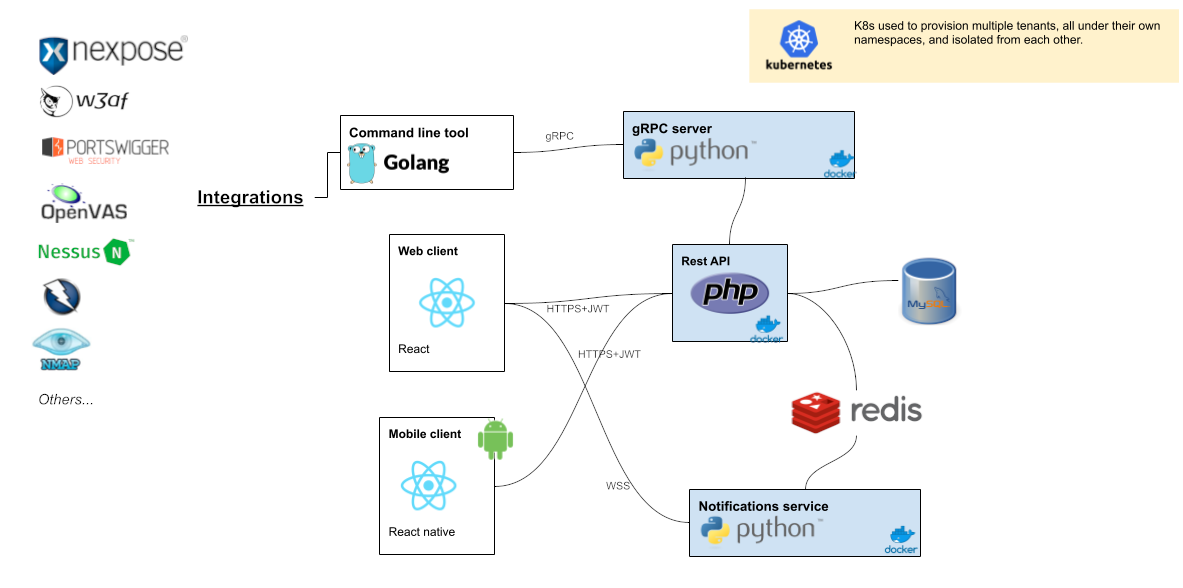
\includegraphics[]{reconmap-architecture.png}
\end{frame}

\begin{frame}
    \frametitle{API}

    \note[item]{
    }

	\begin{itemize}
		\item RESTful API
		\item OpenAPI specs
		\item Fully featured
		\item Used by CLI, Web and mobile clients
		\item \url{https://api.reconmap.org/docs/}
	\end{itemize}
\end{frame}

\subsection{Typical workflow}

\begin{frame}
    \frametitle{Typical workflow}

    \note[item]{
    }
    
    \begin{enumerate}
    \item Create client
    	\item Create project from template
    	\item Complete tasks
    	\item Some tasks require running commands
    	\item Reconmap (\textit{rmap}) runs the command, upload results, and analyses them
    	\item User annotates and triage vulnerabilities
    	\item Generate and share the report
    \end{enumerate}
\end{frame}



\section{Reconmap's interactive demo}

\begin{frame}
    \frametitle{Reconmap's demonstration}

    \note[item]{
    }

    \begin{itemize}
    		\item General tour
    		\item Pentest generation walk-through
    \end{itemize}
\end{frame}

\subsection{Present and future}

\begin{frame}
    \frametitle{Reconmap's present}

    \note[item]{
    }
    
	\begin{itemize}
		\item Young project ($\sim$ 7 months, part-time)
		\item Usable, but not complete
		\item Evolving fast (releases every 2 weeks)
	\end{itemize}
\end{frame}

\begin{frame}
    \frametitle{Reconmap's future}

    \note[item]{
    }

	\begin{columns}
		\begin{column}{0.5\textwidth}
	\begin{outline}
		\1 Immediate term
			\2 Polish up
			\2 Expand docs
			\2 Expand test coverage
	\end{outline}
		\end{column}

		\begin{column}{0.5\textwidth}
	\begin{outline}
		\1 Short term
			\2 Add more integrations
			\2 2FA
			\2 Item triage
			\2 Better analytics
	\end{outline}
		\end{column}
	\end{columns}
\end{frame}

\begin{frame}
    \frametitle{Reconmap's future}
    \framesubtitle{Medium term}

    \note[item]{
    }
    
	\begin{itemize}
		\item Machine learning for classification
		\item Non-interactive agents
		\item Many other things!
	\end{itemize}
\end{frame}


\begin{frame}
    \frametitle{Recap}

    \note[item]{
    }

    \tableofcontents
\end{frame}

\begin{frame}
    \frametitle{More information}

    \note[item]{
    }

	\begin{description}[style=nextline]
	   \item[Documentation] \url{https://reconmap.org}
	   \item[SaaS] \url{https://reconmap.com}
	   \item[Code] \url{https://github.com/reconmap}
	   \item[Twitter] \url{https://twitter.com/reconmap}	   
	\end{description}
\end{frame}

\section{Q\&A}
\begin{frame}<presentation:1>[noframenumbering]
	\begin{Huge}
	Questions?
	\end{Huge}
\end{frame}

\end{document}
